% Drawing 83/03-1 -- folder 83, batch 03, archive page 45 (PDF page 46).
% Transcription: un carré dont les sommets sont joints par les deux diagonales en pointillé, marqué $Q_1$ et $Q_2$, avec une flèche vers $Q_1$ ; à côté : « On a le troisième coin »
% Kind: square with dotted diagonals. Method 2 (schematic redraw from the facsimile). Status: ok.
% Notes: Square (sides inked heavily) with its two diagonals dotted and dotted inner lines; Q_2 inside, an arrow from the upper left to Q_1. The words "On a le troisieme coin" beside it are text, not drawn.
% Coordinates: 1 unit = 1 mm = 1/100 of the crop width (bbox in page fractions: [0.68, 0.24, 0.86, 0.37]).
% Redrawn by Claude (claude-opus-5-5), issue #73, 2026-11-07; not checked by a human; not compiled (no TeX in the session).
% Rights: reproduces part of the work -- behind RENDER_TRANSCRIPTS, never published by itself.
\documentclass[tikz,border=3pt]{standalone}
\usepackage{amsmath,amssymb}
\usetikzlibrary{patterns,arrows.meta}
\tikzset{pencil/.style={black!45}, struck/.style={black!35}, mark/.style={circle,draw,inner sep=1.3pt}, pt/.style={circle,fill,inner sep=0.9pt}, opt/.style={circle,draw,fill=white,inner sep=1.1pt}}
\begin{document}
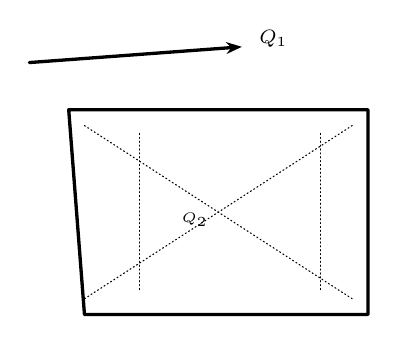
\begin{tikzpicture}[x=1mm,y=1mm,line cap=round,line join=round,font=\scriptsize]
\draw[very thick] (38,-31) -- (76,-31) -- (76,-57) -- (40,-57) -- cycle;
\draw[densely dotted] (40,-33) -- (74,-55);
\draw[densely dotted] (74,-33) -- (40,-55);
\draw[densely dotted] (47,-34) -- (47,-54);
\draw[densely dotted] (70,-34) -- (70,-54);
\draw[-{Stealth[length=2mm]},very thick] (33,-25) -- (60,-23);
\node[inner sep=1pt] at (64,-22) {\scriptsize $Q_1$};
\node[inner sep=1pt] at (54,-45) {\tiny $Q_2$};
\end{tikzpicture}
\end{document}
